\clearpage
\section*{附录B\quad 退化案例的轨迹对照}\label{sec:appendix-trajectories}
\markboth{附录B\quad 退化案例的轨迹对照}{}
\addcontentsline{toc}{section}{附录B 退化案例的轨迹对照}

本附录保留前期状态搜索与强化学习方案的轨迹诊断，所用算法和场景均不属于本节原点扫描版的400个配对场景。两图用于说明早期方案可能出现的绕行现象，不作为新版的轨迹或实验结果。

图\ref{fig:q23-7}为状态搜索相对前瞻基线退化最大的首版随机场景。
图\ref{fig:q23-8}为PPO相对前瞻基线退化最大的场景。
两图均显示全部四方法，不因展示负例而省略其他方法结果。

\begin{figure}[!htbp]
\centering
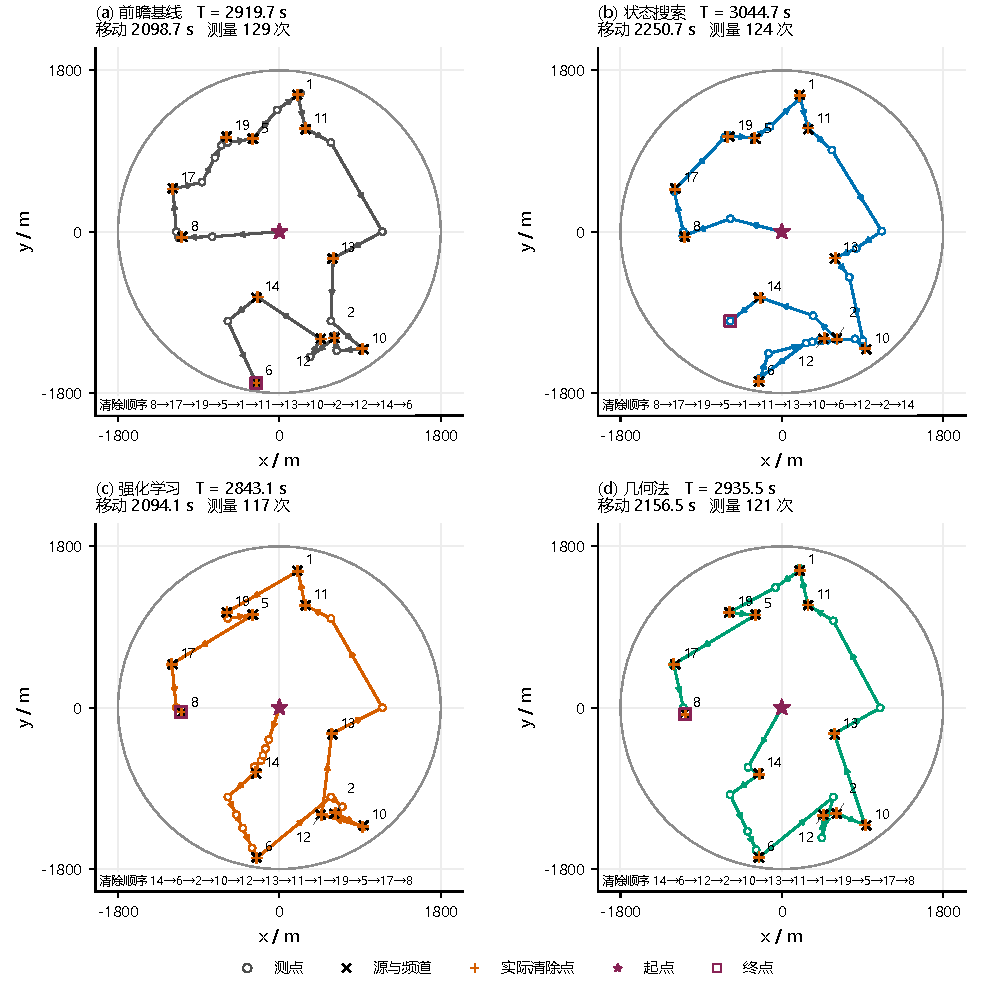
\includegraphics[width=\linewidth,height=\textheight,keepaspectratio,alt={状态搜索最大退化场景800015。状态搜索虽减少检测，却因移动增长而较基线慢125.08 s；此例为事后诊断选择。}]{figures/fig07_trajectory_state_worst.pdf}
\caption{状态搜索最大退化场景800015。状态搜索虽减少检测，却因移动增长而较基线慢125.08 s；此例为事后诊断选择。}
\label{fig:q23-7}
\end{figure}

\begin{figure}[!htbp]
\centering
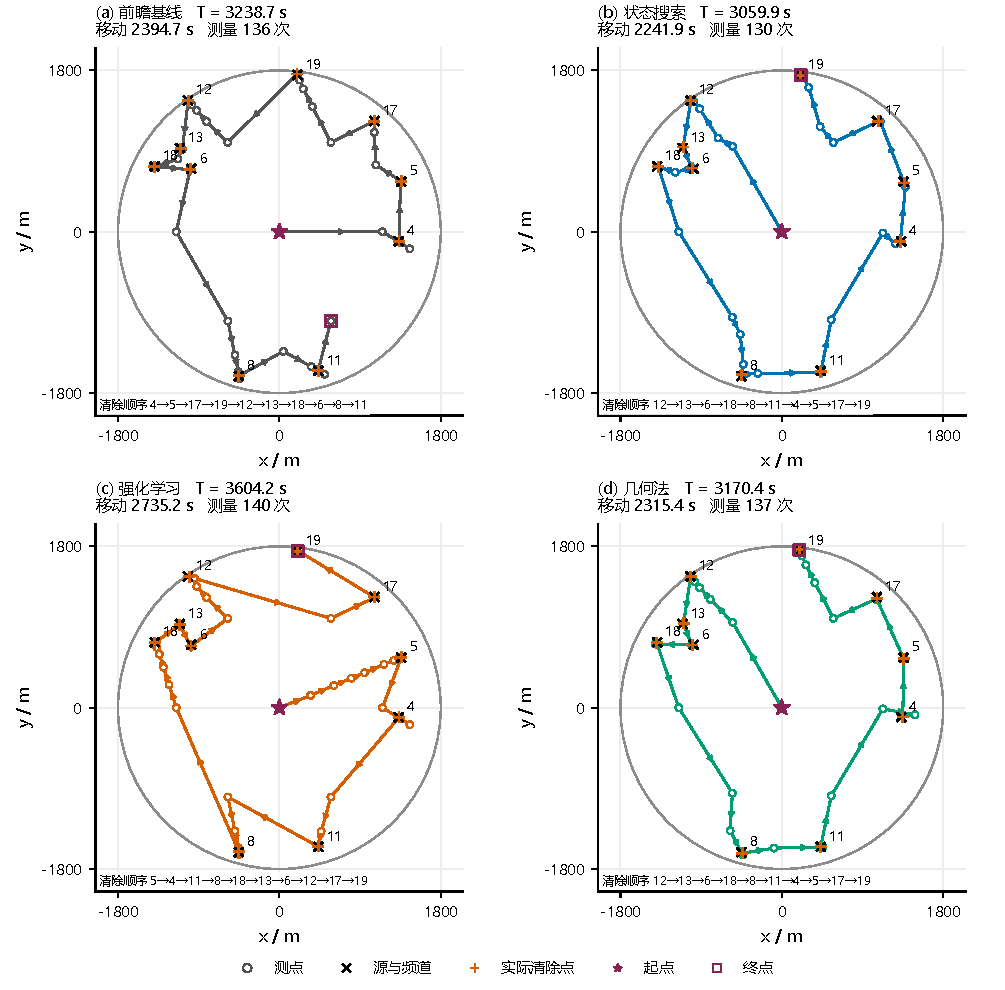
\includegraphics[width=\linewidth,height=\textheight,keepaspectratio,alt={PPO最大退化场景800081。该例主要额外代价来自移动，PPO较基线慢365.45 s；此例不表示总体发生频率。}]{figures/fig08_trajectory_rl_worst.pdf}
\caption{PPO最大退化场景800081。该例主要额外代价来自移动，PPO较基线慢365.45 s；此例不表示总体发生频率。}
\label{fig:q23-8}
\end{figure}

\FloatBarrier

